\section{算术概形}

我们最后一类概形是有限生成约态环但不包含任意域的环的谱。一般地,有限生成$\zz$-代数的谱被称为\textit{算术概形}\index{概形!算术},它们主要在数论中出现,尽管并非所有数论学家感兴趣的概形都具有这种形式。在这些例子中,我们将看到概形在算术以及几何的观点之间的惊人统一的许多线索。\nottran

\subsection{$\spec \mathbb{Z}$}

我们从最明显的例子开始,概形$\spec \zz$. 环$\zz$的素理想当然是$(p)$,其中$p$是素数,以及$(0)$,前者对应于$\spec \zz$的闭点,剩余类域是$\mathbb{F}_p$,后者是一个“一般”点,闭包是整个$\spec \zz$而剩余类域是$\mathbb{Q}$. 图像如下:

% \pic{15.png}

\noindent 这与域上的直线$\mathbb{A}_K^1$在形式上是相似的,事实上,这只是一系列类比的开始,因此在看下面的例子时应将其铭记在心。然而,这种类比也有着它的不足:尽管$\spec \zz$表现得很像$\mathbb{A}_K^1$,但比如$\mathbb{A}_K^1$是$\mathbb{P}_K^1$的稠密开子概形,而$\spec \zz$不是任何一个概形的稠密开子概形。

\subsection{数域中整数环的谱}

其次,考虑概形$\spec A$,其中$A\subset K$是数域$K$中的整数环。作为例子,我们将分析$K=\mathbb{Q}[\sqrt{3}]$以及$A=\mathbb{Z}[\sqrt{3}]$. 正如$\spec \zz$的情况,$\spec A$有两类点,一类对应于$A$的非零素理想,具有有限剩余类域,另一类是一个一般点,对应于$(0)$,剩余类域是$K$. 含入映射$\zz\hookrightarrow A$诱导的映射$\spec A\to \spec \zz$让这个例子变得有趣起来。比如说,考虑点$[(p)]\in \spec \zz$处的纤维,这就是$A$中包含理想$pA\subset A$的所有素理想的集合,它将表现为下面三种方式中的一个(关于这里没解释的材料的一个好的基础参考文献是Serre [1979]):

\begin{compactenum}[(1)]
	\item 如果$p$整除$K$在$\mathbb{Q}$上的判别式$12$,即对$p=2$或$3$,理想$(p)$是$A$中一个理想的平方,我们有
	\[
	2A=(1+\sqrt{3})^2
	\]
	以及,当然,
	\[
	3A=(\sqrt{3})^2.
	\]
	点$(1+\sqrt{3})$和点$(\sqrt{3})\in\spec A$的剩余类环分别为$\mathbb{F}_2$和$\mathbb{F}_3$.

	\item 否则,如果$3$是一个模$p$的二次剩余,于是素理想$(p)$能分解为两个不同素理想的乘积,比如
	\[
	11A=(4+3\sqrt{3})(4-3\sqrt{3})
	\]
	以及
	\[
	13A=(4+\sqrt{3})(4-\sqrt{3}).
	\]
	在这些点的剩余类域依然是元素个数为素数的有限域,分别是$\mathbb{F}_{11}$以及$\mathbb{F}_{13}$.

	\item 最后,如果$p>3$以及$3$不再是一个模$p$的二次剩余,比如$p=5$或者$7$时,理想$pA$依然是素理想,它对应于$\spec A$中的一个点。在这种情况下,剩余类域是$\mathbb{F}_p$的二次扩张,比如在上面的两个例子中是$\mathbb{F}_{25}$以及$\mathbb{F}_{49}$.
\end{compactenum}

一般地,就像这个例子中,如果$K$是一个二次数域,$A$是$K$中的代数整数环,那么包含$Z\subset A$诱导了概形的映射$\psi:\spec A\to \spec \zz$,$\psi$在每一个闭点$(p)\in \spec \zz$处的纤维是下面的可能中的一个:

\begin{compactenum}[(1)]
	\item 一个非约态的点,其坐标环同构于$A/\pp^2$. 它在$\spec \zz$中的像是约态点$\pp$,而剩余类域是$\mathbb{F}_p$,如果$p$在$A$中\textit{分岔},即$pA$是$A$中一个素理想$\pp$的平方。

	\item 两个约态点$\pp$和$\pp'$的并,剩余类域是$A/\pp=A/\pp'=\mathbb{F}_p$,如果$pA$是$A$中两个不同素理想的乘积。

	\item 一个约态点,它的剩余类域$A/\pp$是$\mathbb{F}_p$的二次扩张,如果$p$在$A$中仍然是素的。
\end{compactenum}

在每个例子中,纤维的坐标环作为$\mathbb{F}_p$-代数,维数都是2. 这是因为$A$是一个秩为2的自由$\zz$-模。这里感兴趣的类比是,映射$\spec A\to \spec \zz$与Riemann面的一个分支覆盖(或者更一般地,一个代数闭域,比如$\cc$上的一维概形)。 基本上,我们能将$\spec A$想象成$\spec \zz$的两层覆盖然后在“分岔”素数上分支,比如就像,$\spec \cc[z]$是$\spec \cc[z^2]$的一个双重覆盖,它在原点处分支。对于$\spec \zz$处的点,一个明显的不同是,分岔点处我们有两个不同的重数为1的点,但在不同于分岔点的点$(p)\in \spec \zz$处,我们只有一个重数为1的点,其剩余类域是$\mathbb{F}_p$的二次扩张,这样的点在下图中我们以均匀的灰色点表示:

% \pic{16.png}

一个具有更丰富内容的类比是非代数闭域上的一维概形之间的有限映射。比如考虑映射
\[
	\spec \rr[x][y]/(y^2-x)\to \mathbb{A}_\rr^1=\spec \rr[x],
\]
只看$\mathbb{A}_\rr^1$中那些剩余类域为$\rr$的点,即对实数$\lambda$形如$(x-\lambda)$的点,我们在点$(x)$处有分岔,对$\lambda\neq 0$,$(x-\lambda)$的原像是剩余类域为$\rr$的两个不同的点(若$\lambda>0$)或是一个剩余类域为$\cc$的点(若$\lambda<0$)。

我们通过观察概形$\spec B$,其中$B\subset A\subset K$是数域的一个序,即$K$中的整数环的子环也有着分式域$K$,来进一步深入上面这个类比。举个例子,$A=\zz[\sqrt 3]$以及$B=\zz[11\sqrt 3]$. 上面描述的映射$\spec A\to \spec \zz$现在可以分解为$\spec A\to \spec B\to \spec \zz$,事实上,映射$\spec A\to \spec B$除了两个点$(4+3\sqrt 3)$和$(4-3\sqrt 3)\in \spec A$同时映到$(11,11\sqrt 3)\in\spec B$之外,它就是一个同构。我们于是将$\spec B$画成一种“结点曲线”,即,$\spec A$到$\spec \zz$的双重覆盖中的两点在这里重合了。

% \pic{17.png}

或者,考虑$A=\zz[\sqrt 3]$以及$B=\zz[2\sqrt 3]$的情况。这里映射$\spec A\to\spec B$是一对一的但不是一个同构,点$[(1+\sqrt 3)]$映到了$[(2,2\sqrt{3})]$.

\begin{exe}
	证明,点$p=[(2,2\sqrt{3})]$是概形$\spec \zz[2\sqrt 3]$的一个“尖点”,即这是一个奇异点以及消除奇异性的映射$\spec A\to \spec B$在点$p$处的纤维包含一个二重点。
\end{exe}

\subsection{$\spec \mathbb{Z}$上的仿射空间}

我们下一个例子是一个二维概形$\spec \zz[x]$,或者被记作$\mathbb{A}_\zz^1$. $\zz[x]$中的素理想是
\begin{compactenum}[(i)]
	\item $(0)$;
	\item $(p)$,其中$p\in\zz$是一个素数;
	\item 主理想$(f)$,其中$f\in\zz[x]$是一个$\mathbb{Q}$上的不可约多项式,且所有系数的最大公因子为$1$;
	\item 极大理想$(p,f)$,其中$p\in \zz$是一个素数,而$f$是一个首一多项式,模$p$后是不可约的。
\end{compactenum}

\begin{exe}
	证明这点。
\end{exe}

这些素理想中,只有最后一类是闭点。第一类的闭包是整个$\mathbb{A}_\zz^1$,第二第三类的闭包我们下面描述。

可能图像化$\mathbb{A}_\zz^1$的最好方式是通过映射$\mathbb{A}_\zz^1\to\zz$(依然是平坦映射!)。在这个映射下, 上面的第二第四类便被映射成$(p)\in\spec \zz$,而第一第三类点将被映射成$\spec \zz$的一般点$(0)$. 实际上,这个映射在点$(p)$的纤维同构于$\mathbb{A}_{\mathbb{F}_p}^1=\spec \mathbb{F}_p$,点$(p,f)\in\mathbb{A}_\zz^1$将对应于多项式$f$在代数闭包$\bar{\mathbb{F}}_p$中的根给出的$\mathbb{A}_{\mathbb{F}_p}^1$中的点(回忆,$\mathbb{A}_{\mathbb{F}_p}^1$中的点对应于Galois群$\mathrm{Gal}\left(\bar{\mathbb{F}}_p/\mathbb{F}\right)$作用在$\mathbb{F}_p$上的轨道)。类似地,一般点$(0)$处的纤维是概形$\mathbb{A}_\mathbb{Q}^1=\spec \mathbb{Q}[x]$,$(f)\in\mathbb{A}_\zz^1$交$\mathbb{A}_\mathbb{Q}^1$于$f$在$\bar{\mathbb{Q}}$中的根对应的点。因此,图像如下:

% \pic{18.png} 
\label{p.2.18}

点$(p)\in\mathbb{A}_\zz^1$的闭包是点$(p)\in \spec \zz$处的纤维$\mathbb{A}_{\mathbb{F}_p}^1$. 其他非闭点,即上面的第三类点,的闭包更有趣。它们将包含点$(f)$本身,它在点$(0)$处的纤维$\mathbb{A}_\mathbb{Q}^1$中,以及所有点$(p,g)\in\mathbb{A}_\zz^2$,其中$g$是$\bar{\mathbb{F}}$上$f$的一个因子,即对$\mathbb{A}_\zz^1$的每一条纤维$\mathbb{A}_{\mathbb{F}_p}^1$,$\mathbb{A}_{\mathbb{F}_p}^1$中点的并对应于$f$模$p$后的根。

\begin{exe}
	在上图中打问号的点是上面?为什么点$(4x+1)$以及$(x-2)$的闭包是相切于点$(3,x-2)$且都横截$(3)$的闭包的那两条曲线?(一个答案见到Exercise \ref{e.2.44}前的讨论。)为什么点$(4x+1)$的闭包画出来在点$(2)\in\spec \zz$上有一个竖直的渐近线?
\end{exe}

另一个例子,考虑由一个单线性多项式生成的理想,比如$(5x-49)$. 为了继续$\spec \zz$与域上的仿射直线的类比,我们把该点的闭包想象成$\spec\zz$上函数$49/5$的图像,这是一个在点$(5)$处有一个单极点,在点$(7)$处有一个双重零点的函数。(这条曲线相切于$\mathbb{A}_K^1$的子概形$(x)$,正如下面事实所暗示的那样:$(x)$与子概形$(5x-49)$不止相交于点$(7,x)$,而且还包含一个非约化点支撑于这点。)

点$(x^2-3)$的闭包长得稍微有点不一样,如下图所示:

% \pic{19.png}

\noindent 它的闭包是上面描述过的概形$\spec \zz[x]/(x^2-3)=\spec \zz[\sqrt 3]$,这里被实现为$\mathbb{A}_\zz^1$的一个子概形。

\begin{exe}
	确定上图中三个没有标记的点是什么?
\end{exe}

更一般地,概形$\mathbb{A}_\zz^n=\spec \zz[x_1$, $\dots$, $x_n]$最好通过自然映射$\mathbb{A}_\zz^n\to\spec \zz$来看,它的纤维是概形$\mathbb{A}_{\mathbb{F}_p}^n$以及$\mathbb{A}_{\mathbb{Q}}^n$.

\subsection{$\spec \mathbb{Z}$上的圆锥曲线}\label{sec:2.4.4}

我们的下一个例子给出了概形理论取得的几何与算术的深刻统一性的线索。我们考虑概形
\[
	\spec \zz[x,y]/(x^2-y^2-5),
\]
它同构于$\spec \zz$.

首先,这个概形在一般点$[(0)]\in \spec \zz$处的纤维是概形$X=\spec \mathbb{Q}[x,y]/(x^2-y^2-5)$,我们已经描述过它了:它的点是满足$x^2-y^2=5$的偶对$(x,y)\in \bar{\mathbb{Q}}\times \bar{\mathbb{Q}}$在Galois群$G=\mathrm{Gal}(\bar{\mathbb{Q}}/\mathbb{Q})$作用下的轨道。类似地,点$(p)$处的纤维是$\mathbb{F}_p$上仿射平面$\mathbb{A}_{\mathbb{F}_p}^2$的由方程$x^2-y^2=5$定义的子概形,即,它的点是满足$x^2-y^2=5$的偶对$(x,y)\in \bar{\mathbb{F}}_p\times \bar{\mathbb{F}}_p$在Galois群$G=\mathrm{Gal}(\bar{\mathbb{F}}_p/\mathbb{F}_p)$作用下的轨道。

与一般点处的纤维类似,这个概形在除了素数$2$和$5$之外的所有纤维都是非奇异的圆锥曲线。

\begin{exe}
	是否存在$\spec \zz$上的平面圆锥曲线是约化且非奇异的?分类它们。
\end{exe}

然而,$(2)$和$(5)$处的纤维是奇异的:在模$2$的情况下,我们有
\[
	x^2-y^2-5=(x+y+1)^2,
\]
在模$5$的情况下,我们有
\[
	x^2-y^2-5=(x+y)(x-y).
\]
于是$(2)$处的纤维是一条二重直线,而$(5)$处的纤维是两条直线的并(于是特别地,有两个非闭点映射到点$(5)$,而只有一个这样的点映射到其他的$(p)\in \spec \zz$)。

% \pic{20.png}

% \begin{wrapfigure}{r}{160pt}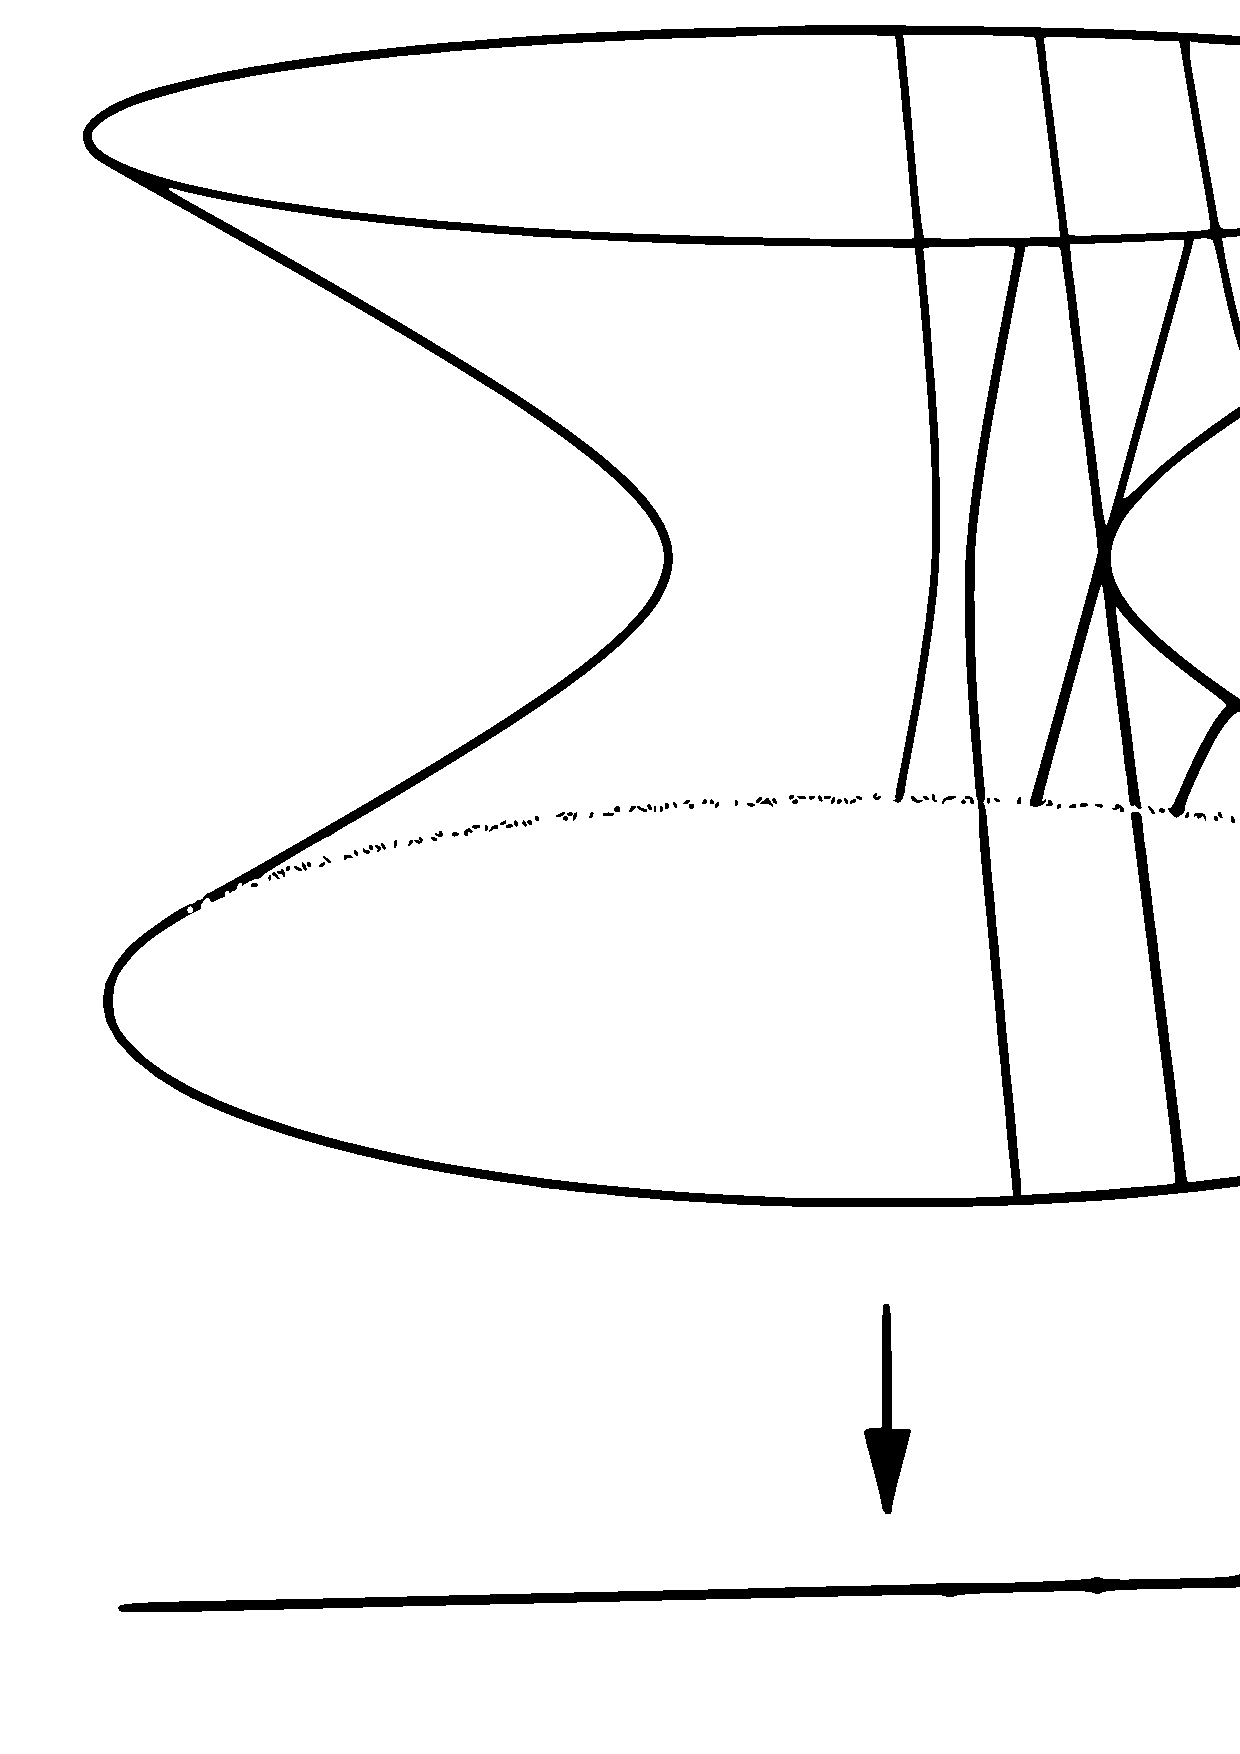
\includegraphics[scale=0.5]{chap_2/pics/21.png}\end{wrapfigure}
\noindent\textbf{Exercise\hspace{0.38em}{\addtocounter{thm}{1}}\thethm.}(这题需要有一定的射影几何知识。)设$(p)\in\spec\zz$满足$p\neq 5$且$p\equiv 1\text{ mod } (4)$,则$X$在点$(p)$上的纤维是一个双曲线,即,它相交于纤维$\mathbb{A}_{\mathbb{F}_p}^2$中“无穷远直线”的两个点,此二点的剩余类域是$\mathbb{F}_p$以及同构于$\mathbb{A}_{\mathbb{F}_p}^1-\{0\}$. 举个例子,若$(p)$上的纤维是曲线$x^2+y^2-5=0$,则它在$\mathbb{F}_p$上的投射平面上的闭包具有方程$X^2+Y^2-5Z^2=0$,于是它在无穷远处交直线$Z=0$于两点$[1,\alpha,0]$,其中$\alpha^2=p-1\text{ mod } (p)$. 证明,与此不同,若$p\equiv 3\text{ mod } (4)$,则纤维是一个椭圆,即,它与无穷远直线相交于一个点,该点处的剩余类域是$\mathbb{F}_{p^2}$. \vspace{0.5em}

上述图像非常符合其几何类比,一个纤维于一条曲线的曲面。比如,曲面$V(x^2-y^2-z)\subset \spec K[x$, $y$, $z]$纤维于$z$-直线$\spec K[z]$。纤维于一条曲线的曲面将具有有限个奇异纤维,正如右边的经典图片所示。

\subsection{$\mathbb{A}_\zz^1$中的双重点}

接着,我们考虑$\zz$上的双重点。再次,令
\[
	X=\bba_\zz^2=\spec\zz[x].
\]
若$Z\subset X$是一个支撑于一点的闭子概形,关联于素理想$(p,f)$,正如在域上的有限子概形那般,我们希望谈论$Z$的度。在域上的概形中,我们定义度为$\oo_Z(Z)$作为$K$-矢量空间的维度。但是现在$\oo_Z(Z)$可能不再能包含任意的域,比如它可能是$\zz/(p^2)$. 更加令人困惑的时候,它的剩余类域可能不是$\zz/(p)$. 因此,摆脱手头这困境最实惠的方式是,首先注意到基数$\# \oo_Z(Z)$一定具有形式$p^d$,进而可以我们可以取度为$d$,显然,如果$\oo_Z(Z)$是一个$\zz/(p)$-矢量空间的话,这就是它的维度。(一个更精致的方法是,先定义约态闭点的度为$\zz/(p)$-矢量空间的维度,然后定义$Z$的度为约态带你的度乘以$Z$在该点的重数。)

比如考虑度为$2$支撑于点$(7,x)$的子概形,它们表现得很像域上的仿射平面上度为$2$的子概形。这样的子概形的理学一定包含极大理想$\pp=(7,x)$的平方,以及同样由$\pp^2$与一个$\pp$中的元素生成,因此
\[
	I=I_{\alpha,\beta}=(49,7x,x^2,\alpha 7+\beta x),
\]
其中$\alpha$, $\beta\in\zz$但不能同时被$7$整除。它只依赖于$\alpha$, $\beta$在$\zz/(7)$中的同余类,同时,将$(\alpha,\beta)$同时呈上$\zz/(7)$中的一个单位将不改变$I$. 因此,对每一个$7$元素域上的投射直线上的点$[\alpha,\beta]$,我们得到了一个支撑于$\pp$的双重点。

\begin{exe}
证明这个对应是双射。
\end{exe}

度为$2$的支撑于$(7,x)$的子概形的集合于是可以等同于域$K=\mathbb{F}_7$上的投射直线$\mathbb{P}_K^1$,就像域$K$上的$\mathbb{A}_K^2$的子概形可以等同于那个域上的投射直线。(在上述任何一种情况下的等同实际上都是将\textit{Zariski切空间}投射到外围空间中。\nottran)然而这有一个不同:$\mathbb{A}_K^2$中所有度为2的支撑于一点的子概形都是同构的,但是由$I_{\alpha,\beta}$定义的子概形$Z_{\alpha,\beta}$看起来是不同,甚至抽象地就可以看出来。若$\beta\neq 0$,我们有
\[
	Z_{\alpha,\beta}=\spec \zz/(49),
\]
但
\[
	Z_{1,0}=\spec(\zz/(7))[x]/(x^2)
\]
与其是不同构的。

\begin{exe}
分类,(a) 度为3且支撑于点$(7,x)\in\mathbb{A}_\zz^1$的子概形,以及(b) 度为4且支撑于点$(2,x^2+x+1)$的子概形。
\end{exe}

\begin{exe}\label{e.2.44}
参照第\pageref{p.2.18}页的图,使用前面的讨论来证明曲线$(4x + 1)$和$(x-2)$相切,而曲线$(4x + 1)$和$(11)$横截。
\end{exe}

最后,这里有一个$\spec \zz$上的平坦族的例子。回忆在上一节中讨论过直线对的族$M\cup L_t$,其中$M$是直线$x=z=0$以及$L_t$是直线$y=z-t=0$. 那里关键的观察是概形$M\cup L_t$的平坦族当$t\to 0$时并不是概形$M\cup L_0$,而是在原点有一个嵌入点的概形。

这里在由$\spec \zz$参数化的族也有着类似的现象。令$U=\spec \zz[7^{-1}]=\spec \zz-\{(7)\}$是点$(7)\in\spec\zz$的补,令
\[
	W=\bba_U^3:=\spec \zz[7^{-1},x,y,z]\subset \bba_\zz^2
\]
是对应的$\bba_\zz^3$的子概形。令$\mathscr{N}$与$\mathscr{L}$是$\bba_\zz^3$中由分别理想$(x,z)$以及$(y,z-7)$给出的闭子概形,再令$\mathscr{N}^*=\mathscr{N}\cap W$以及$\mathscr{L}^*=\mathscr{L}\cap W$. 令$\mathscr{X}^*$是$\mathscr{N}^*$和$\mathscr{L}^*$的并,$\mathscr{X}\subset \bba_\zz^3$是$\bba_\zz^3$中$\mathscr{X}^*$的闭包。于是,我们能把$\mathscr{X}^*$想成由$U$参数化的直线对的族,以及$\mathscr{X}$在点$(7)\in\spec \zz$的纤维$X_7$是这个平坦族“当$7$趋向于$0$”时的极限。正如我们期待的,纤维$X_7$支撑于$\mathscr{N}$与$\mathscr{L}$在点$(7)$处的纤维$(x=z=0)$与$(y=z=0)$的并,但概形$X_7$是非约态的,就像上一节的图片一样,它在原点处有一个嵌入点。

\begin{exe}
验证$\spec\zz$上$\mathscr{X}$的平坦性并描述$X_7$. 你能在$\spec\zz$上找到上节中讨论的其他平坦族的类似物吗?
\end{exe}